
\chapter[Introdução]{Introdução}


\section{Contexto}



A evolução da engenharia de software trouxe à tona debates fundamentais sobre qualidade dos produtos desenvolvidos. Essa discussão tem início em meados dos anos 70 com a criação do primeiro modelo de qualidade conhecido Modelo McCall\cite{mccall1977factors}. Posteriormente, o modelo proposto por \citeonline{boehm1978characteristics}  expandiu essa visão, categorizando os fatores de qualidade em diferentes níveis de abstração: Os fatores de alto nível, como, utilidade (perspectiva de qualidade em uso), Manutenibilidade (perspectiva em qualidade do produto), e portabilidade (perspectiva de adaptação do software para diferentes mudanças). Sendo esses os modelos pilares para consolidação dos modelos subsequentes FURPS e Dromey, culminando, em 2001, a publicação da primeira norma sobre qualidade de software /IEC 9126. O avanço tecnológico e a globalização impulsionaram revisões contínuas desses padrões, resultando na atual normal /IEC 25010, que estabelece os parâmetros contemporâneos para a avaliação de qualidade de software.\cite{miguel2014review}

Embora a ISO/IEC 25010 forneça a fundamentação teórico fundamental para a qualidade, modelos operacionais subsequentes precisaram ser desenvolvidos para suprir a lacuna da extração contínua e automatizada de métricas. Conforme mapeado pela literatura, destacam-se como evolução metodológica modelos como o Quamoco (2012) e o QATCH (2017). Mostram que mesmo após a reformulação da nova ISO/IEC 25010, a tendência é trazer novos modelos ou formas de interpretações de métricas e medidas de qualidade até um definição clara da qualidade de um software.

No contexto de produtos de software direcionados ao cidadão, a garantia de qualidade torna-se um critério crítico. No setor público, a estratégia de terceirização de desenvolvimento é amplamente adotada como meio de otimizar custos e trasnferir a carga de operacionalização técnica para a iniciativa privada. O arcabouço legal primário que rege essas contratações no Brasil é a Nova lei de Licitações e Contratos \cite{brasil2021lei}. Contudo, a delegação de desenvolvimento não isenta a Administração Pública da responsabilidade sobre o resultado. Quando os requisitos de qualidade não são rigorosamente antedidos, o impacto recai de forma direta e imediata sobre o usuário final, comprometendo a prestação do serviço público digital.

Para orientar e padronizar essas contratações, a Secretaria de Governo Digital (SGD) estabeleceu por meio da Portaria número 750 \cite{brasil2023portaria750} - a qual será aprofundada no Capítulo 2. Embora o modelo tente trazer com maior frequência um cálculo adequado para a qualidade código entregue pela contratada \cite[cap. 12]{brasil2023portaria750}, ela ainda se mostra insuficiente para garantir a completude da qualidade de um produto de software, e deixa em aberto para quais modelos de qualidade e a forma como o mesmo será aferido \cite[cap. 2]{brasil2023portaria750}.

Consequentemente, a aplicação rigorosa de modelos de qualidade em contratos de terceirização permanece na dificuldade de estabelecer métricas estritamente objetivas. Essa lacuna operacional e contratual reconduz o setor público aos desafios já debatidos na literatura cientifica: a necessidade de definir métodos inequívocos e auditáveis para mensurar a qualidade de software entregue por terceiros.


\section{Problema}

Aproximadamente entre os anos de 2010 à 2015, as pesquisas em qualidade de software procuraram responder uma lacuna até então em aberto, no que diz respeito à falta de operacionalização dos abstratos conceitos teóricos definidos nos modelos de qualidade de referência \cite{wagner2012quamoco}.Entretanto, devido a diversidade de modelos propostos e também a não completude dos mesmos, gera insegurança para aderência institucional. \citeonline{gorski2006evaluation}, afirma que as decisões de uma contratação e indicadores devem ser menos subjetivos possíveis.

Diante do alto nível de abstração conceitual dos modelos de qualidade de referência como a ISO/IEC 25010 \cite{iso25000public} e de outros modelos presentes na literatura, o modelo de contratação da SGD delega a operacionalização e definição de medidas e indicadores para o gestor do contrato. Conforme descrito em sua Seção 5.1.6, a definição da metodologia para a aferição da qualidade do produto de software foca sob a responsabilidade da própria contratante. O mesmo prevê como alternativa a contratação de outra empresa para aderência de qualidade. O reflexo disso está no cálculo de indicadores sobre qualidade de código que caracteriza os requisitos de qualidade por parte da contratante.
 
\section{Questão de Pesquisa}

A definição da questão de pesquisa foi elaborada utilizando a abordagem \textit{Goal Question Metric (GQM)}. Essa tem como objetivo definir de forma hierárquica, os objetivos a serem alcançados, as perguntas a serem respondidas para cumprir tais objetivos e as métricas necessárias para responder a cada pergunta de forma quantitativa. Considerando essa perspectiva definimos a seguinte questão principal de pesquisa deste estudo:

\begin{center}
	\textbf{Como operacionalizar os atributos de qualidade de Manutenibilidade, especialmente Analisabilidade e Testabilidade, por meio de indicadores objetivos, para apoiar a aceitação de versões de produtos de software desenvolvidos por terceiros no contexto da fiscalização de contratos públicos de desenvolvimento de software?}	
\end{center}

\begin{table}[!h]
    \centering
    \caption{GQM Adaptado}
    \label{tab-GQM}
    \begin{tabular}{l|p{10cm}}
        \hline
        \textbf{Característica} & \textbf{Valor} \\
        \hline
        Analisar & Produto de software tercerizado \\
		\hline
        Com propósito de & Caracterizar a aceitação de versões de produtos de software  \\
		\hline
        Com respeito ao & A característica de qualidade do produto  Manutenibilidade e suas sub características ( Modularidade e Testabilidade )  \\
		\hline
		Do ponto de vista de & Pesquisador \\
		\hline
		No contexto do  & Fiscalização na entrega de versões do produto, desenvolvido no âmbito da terceirização em contratos de desenvolvimento de software. \\
		\hline
    \end{tabular}
\end{table}



\section{Objetivo}

O objetivo geral deste trabalho é avaliar a qualidade do produto Agenda DF, no contexto da terceirização do Governo do Distrito federal. Para alcançar esses objetivos, foram definidos os seguinte objetivos específicos:

\begin{enumerate}
	\item Fundamentar teoricamente os conceitos de qualidade de software.
	\item Fundamentar sobre o contexto institucional de contratação de desenvolvimento de software.
	\item Planejar um estudo de caso focado em observar a aceitação de versões de produto de software apoiado em evidências quantitativas e qualitativas de medidas e indicadores de qualidade.
	\item Conduzir o estudo de caso, realizando a coleta de métricas, medidas e características no que diz respeito a Manutenibilidade.
	\item Apresentar as conclusões desta investigação.
\end{enumerate}

\section{Composição e estrutura do trabalho}

O presente trabalho está organizado em quatro capítulos, conforme descrito a seguir.

O \textbf{Capítulo 1 — Introdução} apresenta o contexto que motivou a pesquisa, situando a problemática da qualidade de software no âmbito das contratações públicas de desenvolvimento. São definidos o problema de pesquisa, a questão principal orientada pelo framework \textit{Goal Question Metric} (GQM), os objetivos geral e específicos, e a composição do trabalho.

O \textbf{Capítulo 2 — Referencial Teórico} consolida os conceitos fundamentais que sustentam a investigação. São abordados os principais modelos de qualidade de software — de McCall (1977) e Boehm (1978) à norma ISO/IEC 25010 — com ênfase nos atributos de Manutenibilidade, Modularidade e Testabilidade. Complementarmente, são discutidos o arcabouço legal das contratações públicas de TI no Brasil, incluindo a Lei n\textordmasculine\ 14.133/2021 e a Portaria SGD/MGI n\textordmasculine\ 750/2023, e os desafios inerentes à terceirização de desenvolvimento de software.

O \textbf{Capítulo 3 — Revisão Estruturada da Literatura} descreve a condução da revisão bibliográfica sistemática realizada para responder às sete questões secundárias de pesquisa. São apresentados o protocolo baseado em \citeonline{kitchenham2007guidelines}, a \textit{string} de busca elaborada com o protocolo PICO adaptado, os critérios de seleção e os resultados da análise dos 30 artigos incluídos na leitura completa.

O \textbf{Capítulo 4 — Planejamento do Estudo de Caso} detalha o delineamento metodológico da etapa empírica do trabalho. São definidos o objeto de estudo, o protocolo de coleta e análise de métricas de qualidade, e os instrumentos que orientarão a condução da investigação sobre o produto de software Agenda DF no contexto do Governo do Distrito Federal.

Por fim, os elementos pós-textuais compreendem as referências bibliográficas, os apêndices e os anexos pertinentes ao trabalho.

\section{Cronograma e Atividades}

\subsection{Primeira etapa}

Nesta é detalhado a primeira etapa da monografia, que consiste no levantamento inicial do problema a ser explorado, e a definição da proposta empírica. Abaixo temos o Cronograma correspondentes


\begin{figure}
	\centering
	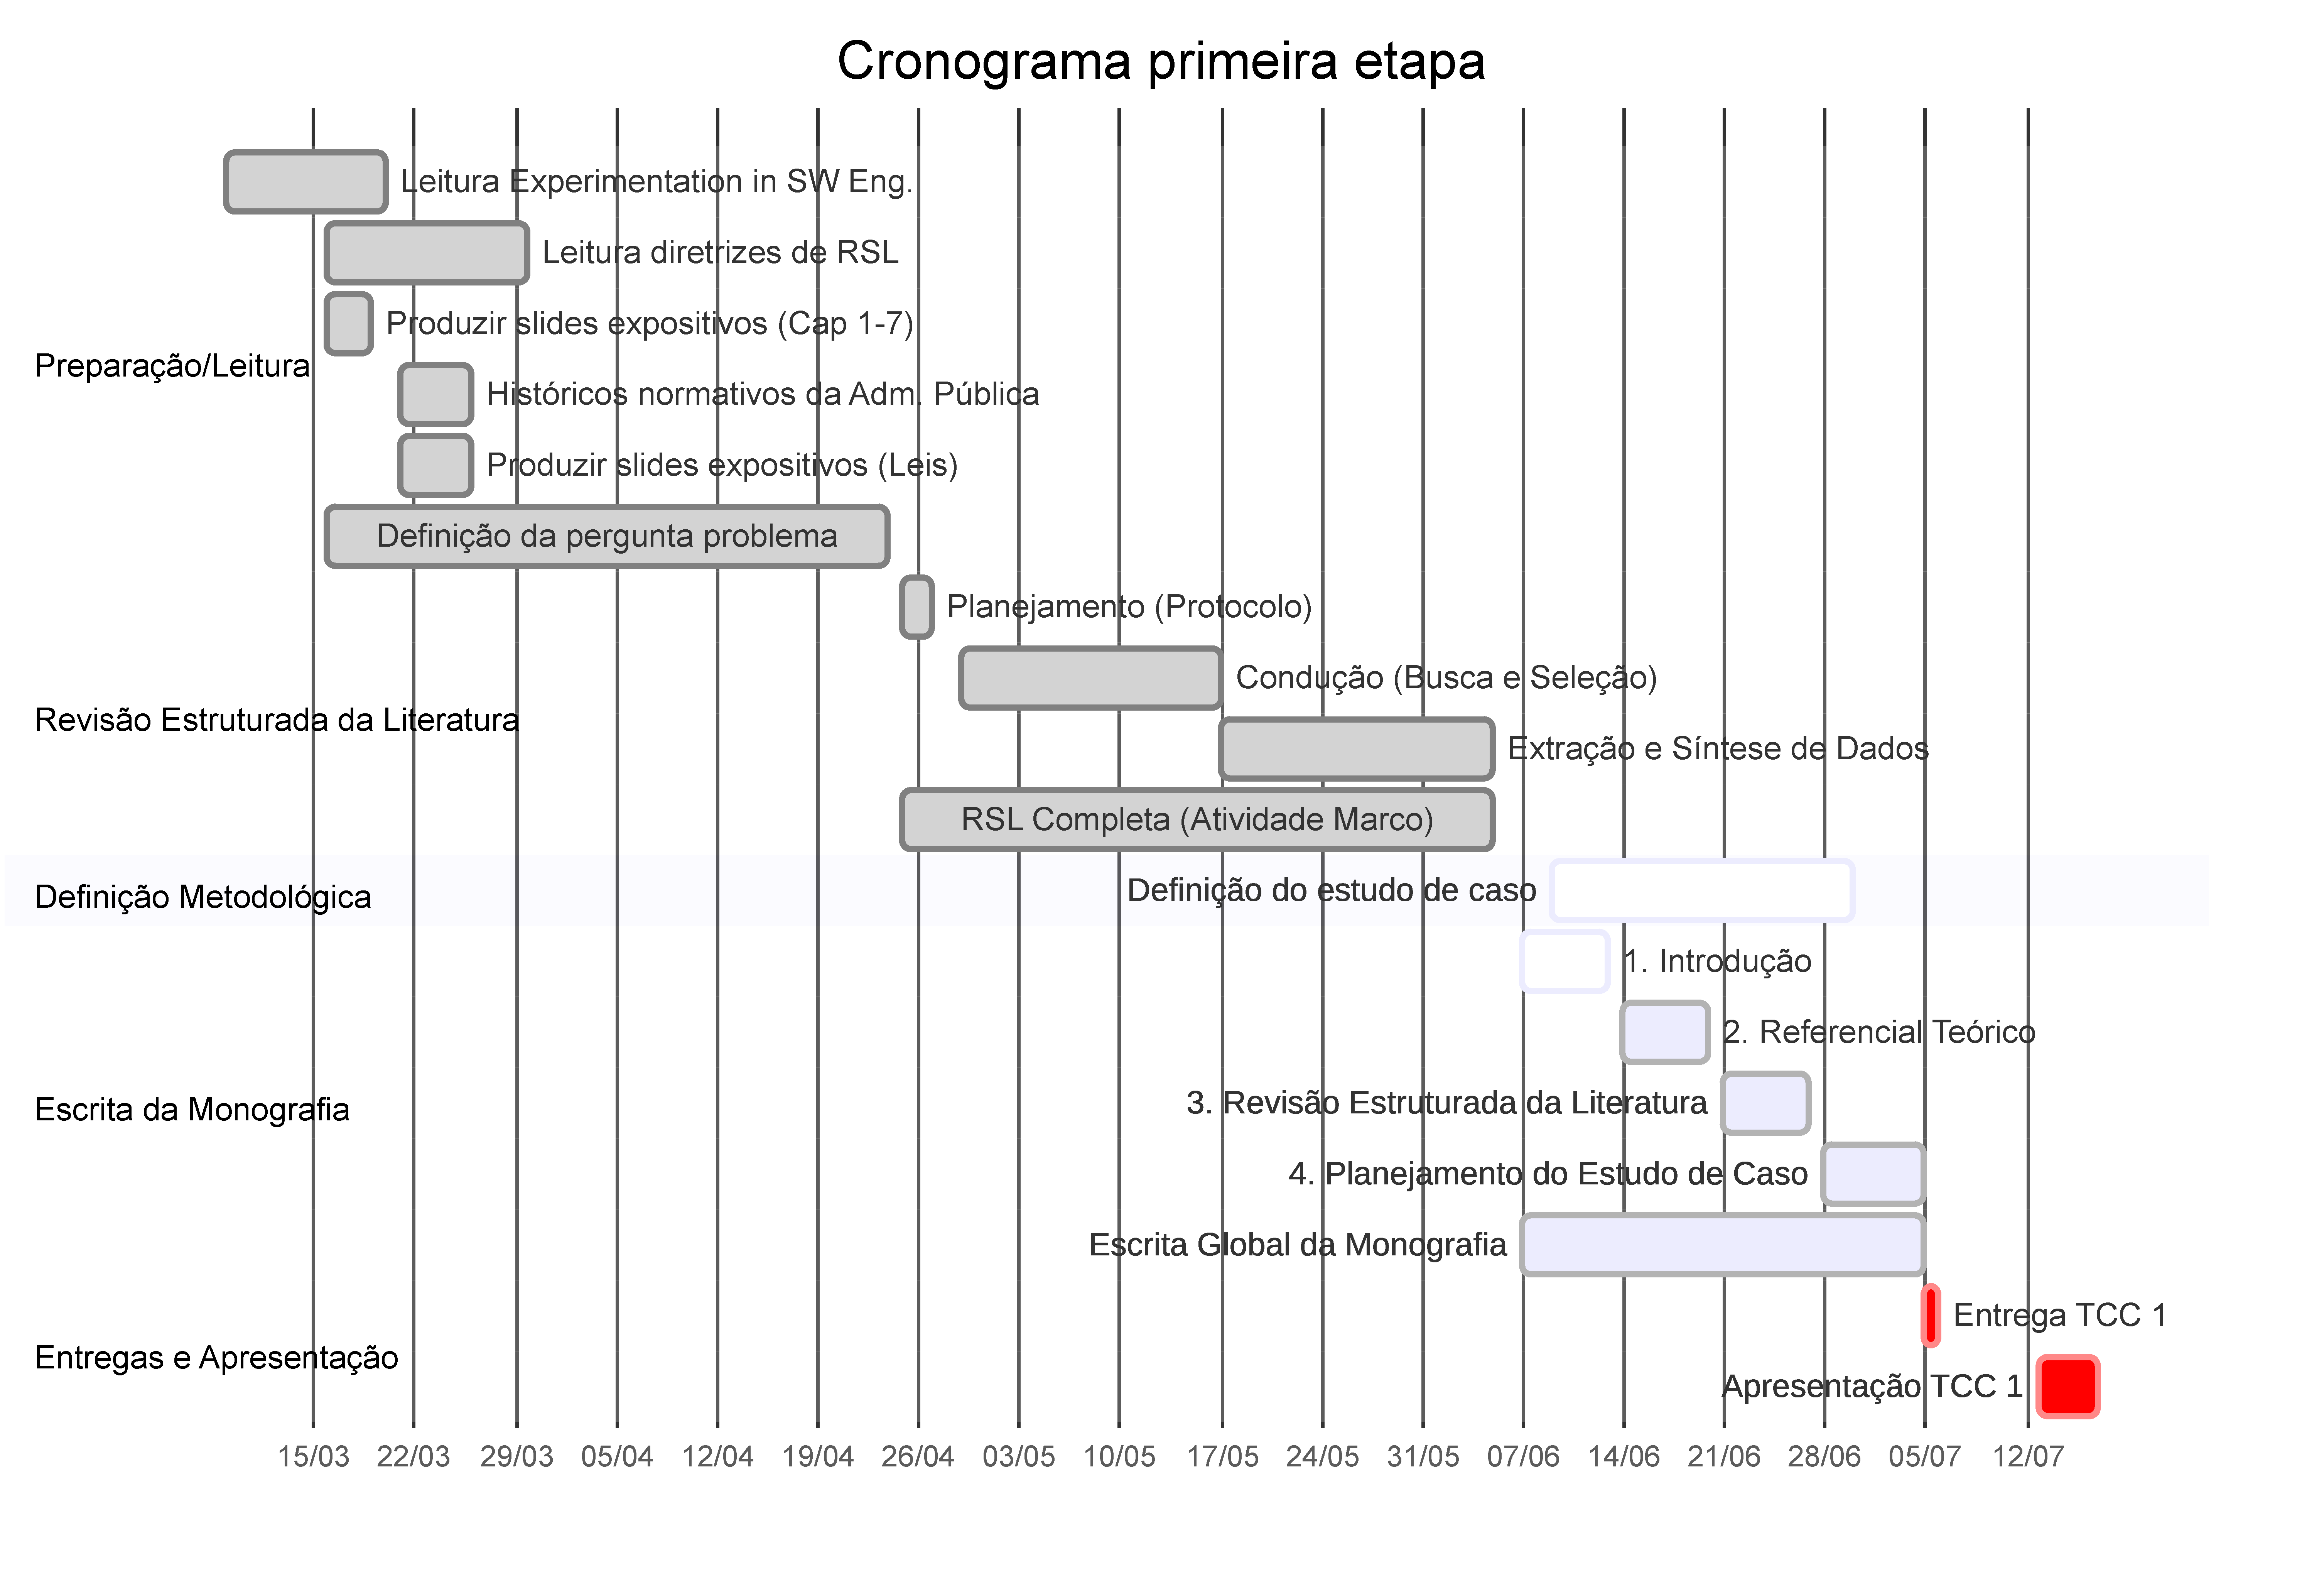
\includegraphics[width=0.8\textwidth]{figuras/cronograma-primeira.pdf}
	\caption{Cronograma de atividades}
	\label{fig-cronograma}
\end{figure}



\begin{enumerate}
	\item Contextualização sobre engenharia de software experimental, entendimento geral dos principais métodos utilizados e pesquisas empíricas, em especial a revisão sistemática da literatura, o estudo de caso, entrevista e questionários que serão fundamentais para a condução do trabalho proposto.
	\item Definição do GQM, apoio para a construção da pergunta principal de pesquisa.
	\item Elaboração do protocolo de revisão da literatura, estruturado e adaptado do protocolo de revisão sistemática da literatura, proposto por \citeonline{kitchenham2007guidelines}. Essa sistematização organizará nossos processo de revisão da literatura pertinente.
	\item Seleção dos artigos
	\item Análise do material selecionado
	\item Definição da proposta de solução
	\item Redação da monografia
	\item Revisão
	\item Defesa
\end{enumerate}


